\chapter{Avaliação e Resultados}\label{cap3}

O \autoref{cap2:treplica_reconfiguravel} apresentou três funcionalidades para expansão da
biblioteca Treplica:

\begin{enumerate}
  \item Protocolo para transferência de estado: criação de um mecanismo eficiente para
    transferência de estado entre réplicas.
  \item Réplicas leitoras: possibilidade da utilização de réplicas que não participam do
    processo de decisão de instâncias de consenso.
  \item Equalização de estado: proposta para novo componente de preenchimento de lacunas
    originadas por possíveis períodos de instabilidade da réplica e/ou falhas.
\end{enumerate}

Supomos duas hipóteses baseado-se nas alterações propostas 1 e 2. A alteração proposta
pelo item 3 não será validada por esse trabalho. Mantivemos a descrição dessa alteração
para enriquecimento do conteúdo e possível utilização em trabalhos futuros.

\begin{enumerate}
  \item Se possuirmos um mecanismo transferência eficiente, podemos recuperar o estado de
    uma réplica de forma mais eficiente que a aplicação do histórico de decreto do
    aglomerado. Lembrando que, toda réplica votante armazena em memória persistente
    qualquer alteração realizada no seu estado.
  \item Se possuirmos uma réplica que evite a reconfiguração total do sistema, ganharemos
    o poder de manobra necessário para expansão do aglomerado de acordo com a demanda de
    clientes.
\end{enumerate}

Para validar que a hipótese 1 e 2 podem aumentar o desempenho de um sistema que utiliza a
biblioteca Treplica, supomos uma carga de trabalho na qual uma parcela significativa das
requisições solicitadas para aplicação seja de leitura. Essa é uma suposição razoável para
a maioria das aplicações de Internet \cite{tpc02} e proporciona o cenário, que acreditamos
ser o mais adequado, para execução eficiente utilizando réplicas leitoras.

Começamos esse capítulo com a \autoref{sec:aplicacao}, apresentando os detalhes da
aplicação e as bibliotecas utilizadas para sua concepção. Em seguida, na
\autoref{sec:ambiente_experimental} descrevemos o ambiente experimental usado na execução
dos experimentos. As próximas duas seções \autoref{sec:experimento_tranferencia_estado} e
\autoref{sec:experimento_replicas_leitoras} apresentam respectivamente os experimentos de
transferência de estado e réplicas leitoras com seus respectivos cenários, resultados e
análise. Encerramos o capitulo com a \autoref{sec:conclusao} apresentando as considerações
finais.


\section{Aplicação}\label{sec:aplicacao}

Para fins experimentais, desenvolvemos então, visando a validação do conjunto de
experimentos, uma aplicação Web simples que mapeia uma cadeia de caracteres para um valor
numérico de 32 bits. Em outras palavras, criamos uma aplicação caracterizada como um mapa
que disponibiliza dois serviços aos clientes remotos através de uma interface HTTP:

\begin{enumerate}
  \item Operação GET \verb|/replicated-map/map/key/<chave>|
  \item Operação PUT \verb|/replicated-map/map/key/<chave>/value/<valor>|
\end{enumerate}

A operação GET é uma operação de leitura, sua função proporciona ao cliente buscar o valor
armazenado em uma determinada chave. Definimos que uma operação bem-sucedida no método GET
retorna o código de status HTTP 200 e um JSON com o valor da chave requisitada
\verb|{"value":"<valor>"}|. Por outro lado, o método PUT defini operações de escrita, ele
é responsável por armazenar um valor em uma determinada chave. Definimos que uma operação
de escrita sem falhas não possui corpo de retorno, o método retorna apenas o código de
status HTTP 201.

Utilizamos a linguagem Scala\footnote{\url{http://www.scala-lang.org}} para criação da
aplicação, sendo que o estado da aplicação é gerenciado pela biblioteca Treplica que atua
como um \emph{middleware} de replicação ativa, conforme ilustra a
\autoref{fig:treplica_como_middleware}. Treplica é uma biblioteca Java e mostrou boa
interoperabilidade com a aplicação. Não relatamos nenhum problema oriundo da utilização de
bibliotecas Java com a linguagem Scala.

\begin{figure}[ht]
  \centering
  \includegraphics[width=12cm]{conteudo/capitulos/figuras/block-treplica.eps}
  \caption{Treplica como \emph{middleware} de replicação ativa}
  \label{fig:treplica_como_middleware}
\end{figure}

Apesar da simplicidade encontrada na aplicação de teste, ela é executada em um aglomerado
de máquinas e oferece pra seus clientes, a garantia de que toda operação de escrita será
replicada para outras instâncias de forma ativa. Com base nessa propriedade, garantimos a
elegibilidade dessa aplicação para execução de experimentos no modelo computacional
utilizando replicação ativa.

Cada uma das réplicas instanciadas possui seu próprio estado e podem assumir diferentes
graus de persistência para dos dados em memória, definido-as como réplicas votantes ou
réplicas leitoras:

\begin{itemize}
  \item Réplica votante: utiliza memória persistente, premissa do algoritmo Paxos para
    garantia de correção no modelo computacional falha-e-recuperação.
  \item Réplica leitora: utiliza memória volátil.
\end{itemize}

\subsection{Dependências}

A \autoref{tab:dependencias} lista as bibliotecas dependentes, com a respectiva versão
utilizada, utilizadas para compilação e execução da aplicação. A tabela lista também a
responsabilidade que a biblioteca exerce no projeto.

\begin{table}[htb]
\IBGEtab{
  \caption{Tabela de dependência de bibliotecas}
  \label{tab:dependencias}
}{
  \begin{tabular}{ccc}
  \toprule
    Biblioteca & Versão & Responsabilidade \\
  \midrule \midrule
    treplica & 0.3.2 & \emph{midleware} de replicação ativa \\
  \midrule
    vraptor & 3.5.1 & controlador MVC \\
  \bottomrule
\end{tabular}
}{
  \fonte{Produzido pelos autores.}
  \nota{Vraptor: \url{http://vraptor3.vraptor.org}}
  \nota{Model-View-Controller, é um padrão de projeto de software que separa a
  representação da informação da iteração do usuário \cite{alguem}}
}{}
\end{table}

\section{Descrição do Ambiente Experimental}\label{sec:ambiente_experimental}

Os experimentos foram realizados em um aglomerado com 16 nós, interligados através de um
\emph{switch} Ethernet de 1 Gbps. Cada nó possui a seguinte capacidade de processamento:

\begin{itemize}
  \item 1 processador Xeon E5620 (2.4 GHz, 6 \emph{threads});
  \item 12 GB de memória RAM;
  \item 500 GB de armazenamento local (disco 7200 rpm);
  \item Plataforma de 64 bits;
\end{itemize}

Os nós utilizam o sistema operacional GNU/Linux Debian 6.0. A \autoref{tab:aplicativos}
lista os aplicativos e suas respectivas versões que foram utilizados para execução dos
experimentos.

\begin{table}[htb]
\IBGEtab{
  \caption{Tabela de aplicativos utilizados nos experimentos}
  \label{tab:aplicativos}
}{
  \begin{tabular}{ccc}
  \toprule
    Aplicativo & Versão & Descrição \\
  \midrule \midrule
    JVM & HotSpot 64-Bit 1.7.0\_45 & Máquina Virtual Java \\
  \midrule
    Apache Tomcat & 7.0.32 & \emph{Servlet container} \\
  \midrule
    HAProxy & 1.5-dev19 & \emph{HTTP Load balancer} \\
  \bottomrule
\end{tabular}
}{
  \fonte{Produzido pelos autores.}
  \nota{Apache Tomcat: \url{http://tomcat.apache.org}}
  \nota{HAProxy: \url{http://www.haproxy.org}}
}{}
\end{table}

O conjunto de réplicas é gerenciado por um servidor balanceador de carga configurado com
HAProxy, usado para melhorar o desempenho de serviços Web distribuindo requisições entre
vários servidores. Todas as requisições dos clientes passam pelo HAProxy, configurado para
receber e rotear as requisições para as réplicas ativas, usando um algoritmo de
revezamento circular (\emph{round-robin}), como ilustrado na \autoref{fig:setup}. Nessa
configuração os processos clientes não compartilham recursos com os processos da
aplicação, ou seja, ou a instância executa processos clientes ou executa processos da
aplicação.

\begin{figure}[ht]
  \centering
  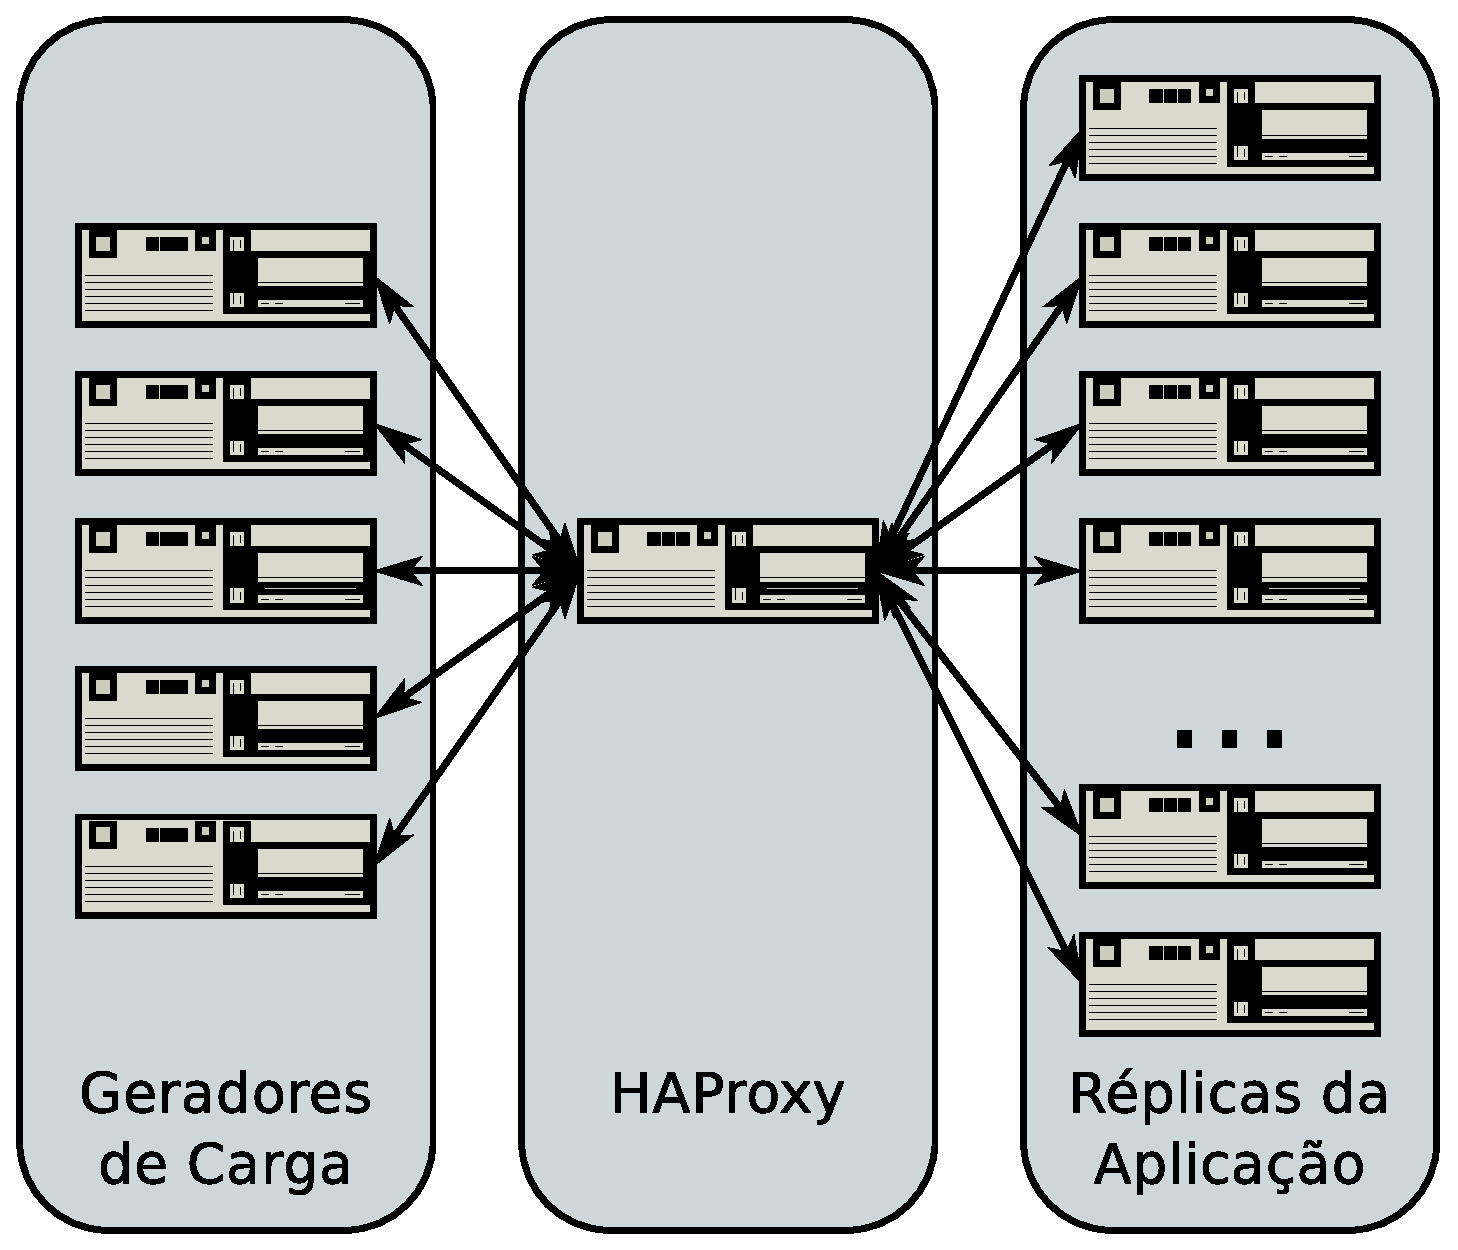
\includegraphics[width=7cm]{conteudo/capitulos/figuras/experimental-setup.dia.eps}
  \caption{Configuração experimental}
  \label{fig:setup}
\end{figure}

\subsection{Carga}\label{subsec:carga}

O programa de teste tem por objetivo produzir a carga de trabalho requirida pelos
experimentos e coletar medidas de vazão do ponto de vista do cliente. Sendo assim, o
programa de teste, em cada instância, registra em \emph{log} o \emph{timestamp} de início
e fim de cada atividade para que seja possível o computar a vazão alcançada pela
aplicação.

Para geração da carga de trabalho utilizamos processos Java que executam requisições de
leitura (requisições para o método HTTP GET) e escrita (requisições para o método HTTP
PUT) respeitando um percentual configurável para realização de cada operação. Para todos
os experimentos dedicamos 5 máquinas para atuarem como clientes, sendo que cada uma
executa 1000 requisições/segundo, variando (sem garantia de ordem) entre requisições de
leitura e escrita.

Do ponto de vista da aplicação, requisições de leitura serão atendidas localmente por uma
das réplicas, enquanto uma requisição de escrita será transformada em uma proposta e
submetida a uma rodada de consenso entre as réplicas votantes. Avaliando-se o custo de
cada tipo de requisição, podemos afirmar que requisições de escritas são mais caras porque
envolvem mais trocas de mensagens que requisições de leitura.

Para execução de todos os experimentos foi gerado uma carga total para aplicação de 5000
requisições/segundo. O tempo total de execução de cada experimento foi de 300 segundos.
Para a análise resolvemos considerar intervalos diferentes de acordo com o cenário de
teste. Tal intervalo, ao qual chamaremos de \emph{período de análise}, será identificado
em cada análise. Visando facilitar a comparação dos experimentos, eles foram divididas em
duas configurações, conforme mostra os dados na \autoref{tab:configuracao_experimento}.

\begin{table}[htb]
\IBGEtab{
  \caption{Configuração da carga experimental}
  \label{tab:configuracao_experimento}
}{
  \begin{tabular}{cccc}
  \toprule
  Experimento & Requisições por segundo & Total de escrita & Total de leitura \\
  \midrule \midrule
  1           & 5000                    & 2500 (50\%)      & 2500 (50\%)      \\
  \midrule
  2           & 5000                    & 1000 (20\%)      & 4000 (80\%)      \\
  \bottomrule
\end{tabular}
}{
  \fonte{Produzido pelos autores.}
}
\end{table}

Identificaremos os experimentos como Experimento 1 e Experimento 2. O objetivo da
configuração do Experimento 1 é criar um cenário que exigirá bastante esforço do protocolo
Paxos devido o equilíbrio da carga de requisições de leitura e escrita. Em contra partida
a configuração do Experimento 2 proporciona um cenário com menos trocas de mensagens
Paxos, já que a maioria das requisições (80\%) são de leitura e são resolvidos localmente
em cada réplica.


\section{Experimento Transferência de Estado}\label{sec:experimento_tranferencia_estado}

Esse experimento está fundamentada na possível disparidade de estado existente entre
réplicas. Para construção desse cenário supomos um aglomerado com cinco réplicas, todas
previamente configuradas com a aplicação de teste. Nosso objetivo é a geração da
divergência do estado replicado em uma das réplicas, para alcançar esse objetivo iniciamos
quatro réplicas simultaneamente e postergamos a inicialização de uma das réplicas.
Definimos então dois instantes no tempo:

\begin{itemize}
  \item $t1$ início da execução das requisições dos clientes;
  \item $t2$ inicialização da aplicação na quinta réplica, $t2$ acontece exatamente 180
    segundos após $t1$.
\end{itemize}

Nessa configuração, o momento $t1$ possui quatro réplicas votantes prontas para atender as
requisições dos clientes e no momento $t2$, a quinta réplica é adicionada ao aglomerado.
Essa nova réplica, poderá ser votante ou leitora dependendo da configuração do
experimento, conforme ilustra a \autoref{fig:timeline}. Do ponto de vista do algoritmo
Paxos, o período entre $t1$ e $t2$ é marcado pela falta de uma réplica, pois devido a
característica estática para definição do total de réplicas, essa propriedade é
previamente definida como cinco antes do inicio da execução.

\begin{figure}[ht]
  \centering
  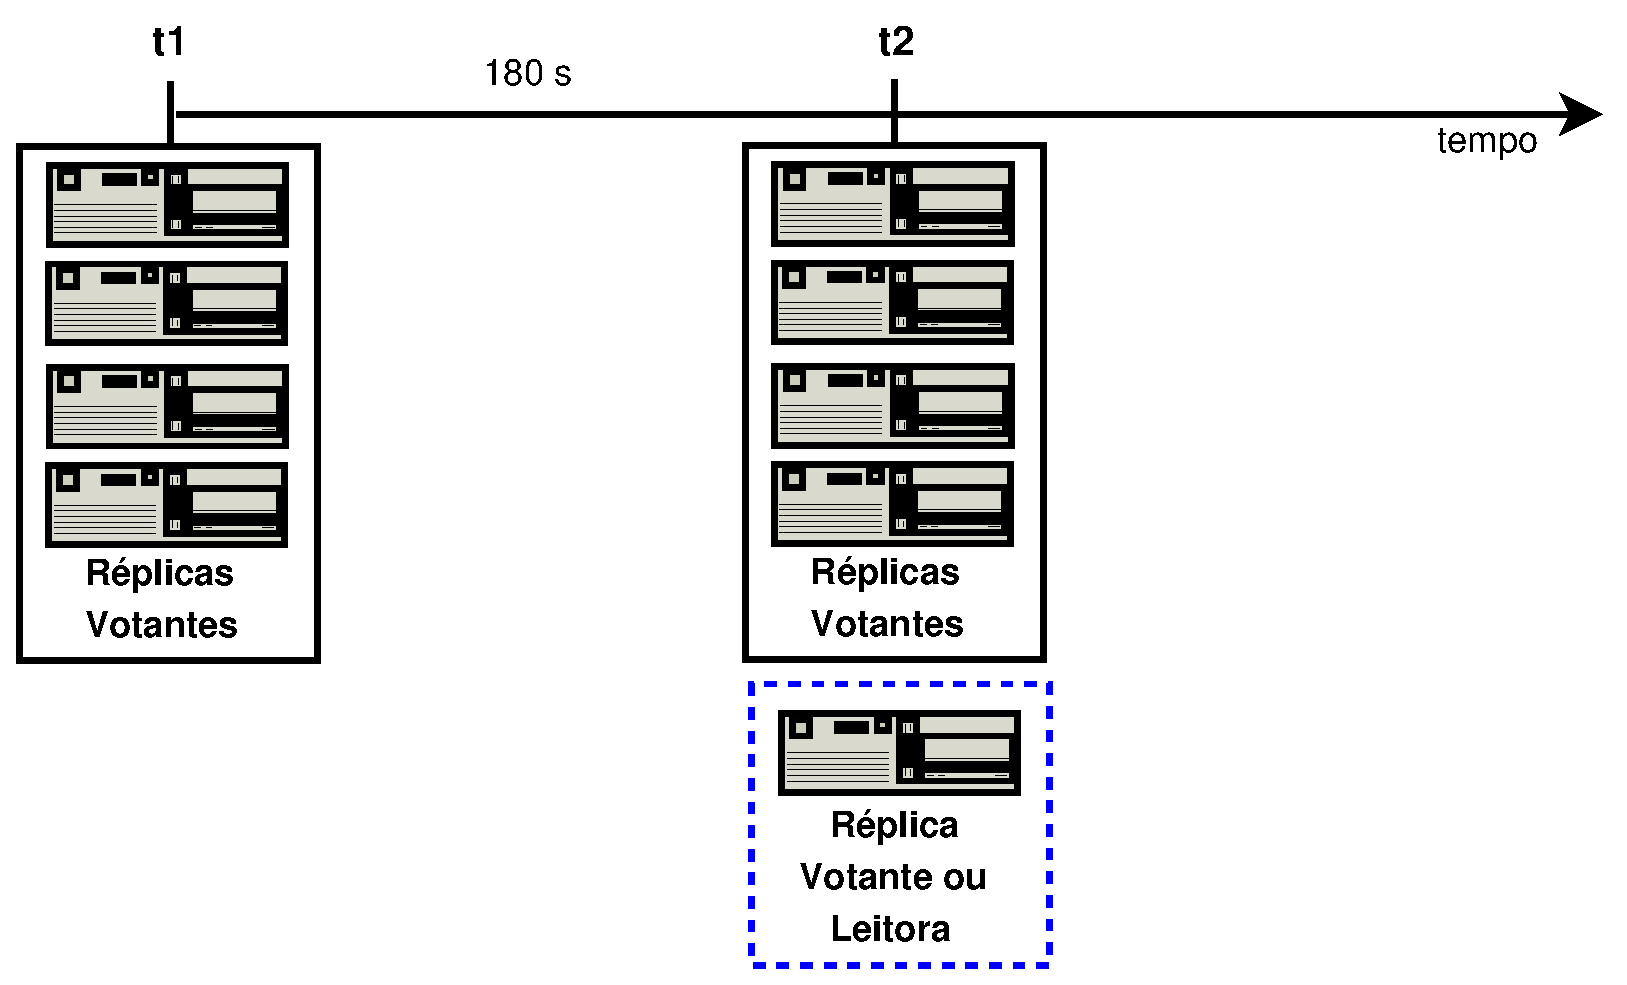
\includegraphics[width=12cm]{conteudo/capitulos/figuras/timeline.eps}
  \caption{Linha do tempo experimento transferência de estado}
  \label{fig:timeline}
\end{figure}

Nesse cenário a formação de quórum para eleição do consenso durante as rodadas de Paxos só
não é legitima quando: (1) No intervalo entre $t1$ e $t2$ duas réplicas falham; (2) Após
$t2$, três máquinas falham.

No entanto, essas restrições só são verdadeiras, se e somente se, a réplica adicionada em
$t2$ é uma réplica votante formando assim um aglomerado de réplicas votantes. Sendo assim,
podemos afirmar que a inclusão de uma nova réplica aumenta a tolerância a falhas da
aplicação e que essa propriedade de sistemas distribuídos, em Treplica, é baseada em
réplicas votantes. A adição de réplicas votantes não altera a tolerância a falhas da
aplicação.

Nessa versão da biblioteca Treplica, o mecanismo de transferência de estado é exclusivo
para réplicas leitoras, abriremos mão da propriedade de tolerância a falhas para
adicionarmos, no instante $t2$, uma réplica leitora para mensurar o impacto causado pela
atuação do protocolo de transferência de estado na aplicação. Para criação de uma base de
comparação, o mesmo teste foi executado adicionando uma réplica votante (sem o mecanismo
de transferência de estado). Nesse caso, a equalização do estado (preenchimento das
lacunas) é realizado pelo mecanismo de retransmissão de instância de consenso já existente
em Treplica.

Notamos nas primeiras execuções do experimento, um estado (em \emph{Megabytes})
relativamente pequeno e pouco atraente para fins experimentais. Essa característica é
resultante da carência de uma carga mais pesada nas requisições de escrita da aplicação
(\autoref{sec:aplicacao}), fator que acarretaria em um aumento mais eficaz do estado.
Sendo assim, do lado do servidor, a cada requisição de escrita associamos uma
\emph{String} de aproximadamente 500 bytes para aumento do estado, conforme ilustra a
\autoref{fig:payload}.

\begin{figure}[ht]
  \centering
  \includegraphics[width=12cm]{conteudo/capitulos/figuras/payload.dia.eps}
  \caption{Carga associada a cada requisição de escrita}
  \label{fig:payload}
\end{figure}

\subsection{Procedimento de teste}

Os passos para execução do experimento de transferência de estado são listados a seguir:

\begin{enumerate}
  \item Iniciar manualmente o serviço do HAProxy em uma instância dedicada para o serviço
    de \emph{load balancer};
  \item Configurar, através de \emph{script}, cinco instâncias que atuarão como
    servidoras, respeitando os parâmetros que define se a réplica atuará como votante ou
    leitora. Nesse passo é executado a instalação da JVM e Tomcat (a aplicação de teste
    foi previamente instalada Tomcat);
  \item Configurar, através de \emph{script}, cinco instâncias dedicadas para o serviço de
    cliente. Nesse passo também é instalado a JVM nas instâncias clientes e o programa de
    teste;
  \item Iniciar com \emph{script} o serviço do Tomcat em quatro réplicas;
  \item Iniciar com \emph{script} o programa de teste nas cinco máquinas dedicadas para
    atuarem como cliente;
  \item Aguardar 180 segundos;
  \item Iniciar com \emph{script} o serviço do Tomcat na quinta máquina (retardatária);
  \item Aguardar mais 180 segundos;
  \item Através de \emph{script}, encerrar os processos Javas iniciados (cliente e
    servidor) e recolher os arquivos de \emph{log} dos clientes e servidores.
\end{enumerate}

\subsection{Resultados e Análise}

A análise de desempenho para esse cenário visa responder duas questões sobre o mecanismo
de transferência de estado em Treplica:

\begin{enumerate}
  \item Qual é o desempenho do mecanismo de transferência de estado?
  \item Qual é a melhor estratégia em Treplica para recuperação de estado: transferência de
    estado ou aplicação uma a uma das instâncias de consenso?
\end{enumerate}

Para responder a primeira pergunta precisamos variar o tamanho do estado para mensurar a
capacidade do mecanismo de transferência. Para criação de tais cenários, combinamos as
configurações do Experimento 1 e do Experimento 2, detalhados na \autoref{subsec:carga},
com a adição de uma réplica leitora, conforme descrito na
\autoref{sec:experimento_tranferencia_estado}. A configuração do Experimento 2 produz um
estado menor (em \emph{Megabytes}) devido a quantidade de requisições de leitura.
Teoricamente esse cenário é favorável para o mecanismo de transferência de estado uma vez
que a quantidade de dados trafegados pela rede é menor.

Estabelecemos os seguintes parâmetros para coleta e medição de desempenho:

\begin{itemize}
  \item Tempo total para envio do estado da réplica receptora para réplica doadora,
    incluindo tempo para estabelecer a conexão TCP entre as réplicas;
  \item Tamanho do estado enviado;
  \item Tempo total para ativação de uma réplica leitora. Essa medida leva em consideração
    o tempo que a réplica demorou para estar apta a processar mensagens da aplicação.
\end{itemize}

A \autoref{fig:dados_transf_estado} (a) exibe o tamanho do estado transferido pelo
Experimento 1 (50\% de requisições de leitura) e pelo Experimento 2 (80\% de requisições
de leitura). O estado do Experimento 1 é desfavorável para ambas as estratégias de
recuperação de estado de Treplica pois produz um estado maior. Comparando os resultados de
tempo de transferência (\autoref{fig:dados_transf_estado} (b)) podemos verificar um melhor
desempenho do Experimento 2 justificada pela diferença no tamanho dos estados nos dois
experimentos. Podemos afirmar então que o desempenho do mecanismo de transferência de
estado está ligado diretamente com o tamanho do estado a ser transferido. Em outras
palavras, quanto maior o estado maior o tempo gasto para transferi-lo.

\begin{figure}[ht]
  \centering
  \includegraphics[width=14cm]{conteudo/capitulos/figuras/dados-transf.eps}
  \caption{Resultado transferência de estado}
  \label{fig:dados_transf_estado}
\end{figure}

Os resultados ilustrado pela \autoref{fig:dados_transf_estado} também são exibidos nas
\autoref{tab:dados_transf_estado1} (Experimento 1) e \autoref{tab:dados_transf_estado2}
(Experimento 2).

\begin{table}[htb]
\IBGEtab{
  \caption{Desempenho da transferência de estado no Experimento 1}
  \label{tab:dados_transf_estado2}
}{
  \begin{tabular}{cccc}
  \toprule
                & Tempo de Transferência & Tamanho do Estado & Tempo de Ativação \\
  \midrule \midrule
  Média         & 1.832s                 & 140.590Mb          & 2.133s            \\
  \midrule
  Mediana       & 1.867s                 & 141.535Mb          & 2.209s            \\
  \midrule
  Desvio Padrão & 0.945                  & 1.934              & 0.631             \\
  \bottomrule
\end{tabular}
}{
  \fonte{Produzido pelos autores.}
}
\end{table}

\begin{table}[htb]
\IBGEtab{
  \caption{Desempenho da transferência de estado no Experimento 2}
  \label{tab:dados_transf_estado1}
}{
  \begin{tabular}{cccc}
  \toprule
                & Tempo de Transferência & Tamanho do Estado & Tempo de Ativação \\
  \midrule \midrule
  Média         & 1.282s                 & 85.096Mb          & 1.533s            \\
  \midrule
  Mediana       & 1.305s                 & 85.150Mb          & 1.513s            \\
  \midrule
  Desvio Padrão & 0.079                  & 0.296             & 0.160             \\
  \bottomrule
\end{tabular}
}{
  \fonte{Produzido pelos autores.}
}
\end{table}

Conforme descrito na \autoref{subsec:funcionamento_protocolo}, o protocolo de
transferência de estado utiliza uma conexão TCP ponto a ponto entre a réplica doadora e
receptora. Essa é uma variável não controlada que pode limitar o desempenho da
transferência de estado. Uma outra possível abordagem, não pertencente ao escopo desse
trabalho é a utilização de um mecanismo colaborativo para envio do estado, onde partes do
estado seriam enviados por diferentes réplicas doadoras, semelhante ao protocolo P2P.
Gostaríamos de saber qual será o impacto que essa abordagem pode causar no desempenho de
Paxos.

A segunda pergunta definida no início dessa seção é referente a escolha da melhor
estratégia de Treplica para recuperação de estado. Para responde-la vamos comparar as
execuções do experimento da \autoref{sec:experimento_tranferencia_estado}, onde
adicionamos ao aglomerado uma nova réplica: ora uma réplica votante ora uma réplica
leitora. O período de análise está concentrado no momento da adição da réplica.
Compararemos os dois mecanismos de recuperação de estado analisando a quantidade de
operações por segundo atendidas em um espaço de 30 segundos de execução. O período de
análise contém registros de 10 segundos antes da adição da réplica e 20 segundos após a
adição.

Continuamos com a mesma configuração de carga definidas pelos Experimento 1 e 2, só que
executados em dois cenários diferentes:

\begin{itemize}
  \item Cenário 1: Execução da carga do Experimento 1 (50\% de requisições de leitura)
    adicionando uma réplica votante e leitora;
  \item Cenário 2: Execução da carga do Experimento 2 (80\% de requisições de leitura)
    adicionando uma réplica votante e leitora;
\end{itemize}

Vamos começar nossa análise pelo Cenário 1. Analisando a
\autoref{fig:transf_estado_cenario1} (a), podemos verificar um grande vale no momento da
adição de uma réplica votante, que chamaremos de $r1$. Assim que o balanceador de carga
detecta que $r1$ está ativa, começa a rotear requisições da aplicação e $r1$ também passa
a receber mensagens do protocolo Paxos oriundas das outras réplicas do aglomerado. Nesse
momento, o mecanismo detector de lacunas de $r1$ também ativo solicitando o histórico de
decisões de consenso do aglomerado. Em outras palavras, o estado do aglomerado está sendo
replicado, instância por instância, em $r1$. A adição de $r1$ causa uma alteração no
desempenho do aglomerado (em termos de operações pro segundo suportada) que é retomado
instantes depois.

Por outro lado, a \autoref{fig:transf_estado_cenario1} (b) ilustra o impacto da adição de
uma réplica leitora $r2$. Podemos verificar uma alteração no número de operações
suportadas quando $r2$ é adicionado. Porém, fica claro que o distúrbio causado pela
adição de uma réplica leitora é menor. Nesse caso, a replicação de estado em $r2$ acontece
através da atuação do mecanismo de transferência de estado. Ou seja, o estado é
transferido em uma única mensagem (\emph{bucket}) causando menos impacto no desempenho do
aglomerado.

\begin{figure}[ht]
  \centering
  \includegraphics[width=14cm]{conteudo/capitulos/figuras/final-transf-estado-pr50.eps}
  \caption{Desempenho da adição de uma nova réplica no Cenário 1}
  \label{fig:transf_estado_cenario1}
\end{figure}

O Cenário 2 está configurado com um maior número de requisições de leitura, a
\autoref{fig:transf_estado_cenario1} ilustra seu desempenho. Mais uma vez podemos observar
menos impacto no número de requisições quando adicionamos uma réplica leitora,
caracterizando assim o bom desempenho do mecanismo de transferência de estado nos dois
cenários experimentais.

\begin{figure}[ht]
  \centering
  \includegraphics[width=14cm]{conteudo/capitulos/figuras/final-transf-estado-pr80.eps}
  \caption{Desempenho da adição de uma nova réplica no Cenário 2}
  \label{fig:transf_estado_cenario2}
\end{figure}

A maior diferença entre a adição de uma réplica votante ou leitora está no tempo de
resposta do período de análise. Nesse caso estamos comparando os mecanismos de
transferência de estado configurado nas duas réplicas. Analisando o resultado ilustrado na
\autoref{fig:analise_final_transf_estado} (a) fica claro, que para esses cenários de
testes a melhor escolha para transferência de estado é a utilização do mecanismo proposto
por esse trabalho. O efeito causado pela redução de mensagens solicitando o envio do
histórico das decisões de consenso também são benéficos quando analisamos o desempenho das
duas estratégias, conforme ilustrado na \autoref{fig:analise_final_transf_estado} (b).

\begin{figure}[ht]
  \centering
  \includegraphics[width=14cm]{conteudo/capitulos/figuras/final-transf-estado.eps}
  \caption{Comparação do desempenho do mecanismo de transferência de estado}
  \label{fig:analise_final_transf_estado}
\end{figure}

Quando comparamos os dois cenários, podemos verificar que o Cenário 2 consegue suportar
mais operações por segundo (\autoref{fig:analise_final_transf_estado} (a)). Isso se deve
ao fato da redução de iterações entre as réplicas requiridas por uma requisição de
leitura, predominante no Cenário 2. Os resultados ilustrado pela
\autoref{fig:dados_transf_estado} também são exibidos na
\autoref{tab:adicionando_replica_votante} (adicionando uma réplica votante) e na
\autoref{tab:adicionando_replica_leitora} (adicionando uma réplica leitora).

\begin{table}[htb]
\IBGEtab{
  \caption{Desempenho para incorporação de uma réplica votante}
  \label{tab:adicionando_replica_votante}
}{
  \begin{tabular}{ccc}
  \toprule
  Leitura & Operações por Segundo & Tempo de Resposta (ms) \\
  \midrule \midrule
  50\%    & 2862.933              & 875.824                \\
  \midrule
  80\%    & 3698.806              & 1095.644               \\
  \bottomrule
\end{tabular}
}{
  \fonte{Produzido pelos autores.}
}
\end{table}

\begin{table}[htb]
\IBGEtab{
  \caption{Desempenho para incorporação de uma réplica leitora}
  \label{tab:adicionando_replica_leitora}
}{
  \begin{tabular}{ccc}
  \toprule
  Leitura & Operações por Segundo & Tempo de Resposta (ms) \\
  \midrule \midrule
  50\%    & 3065.096              & 136.065                \\
  \midrule
  80\%    & 4164.806              & 227.890                \\
  \bottomrule
\end{tabular}
}{
  \fonte{Produzido pelos autores.}
}
\end{table}


\section{Experimento Réplicas Leitoras}\label{sec:experimento_replicas_leitoras}

Para validar a hipótese que réplicas leitoras podem aumentar o desempenho de um sistema
que utiliza Paxos, precisamos de uma carga de trabalho na qual uma parcela significativa
das requisições solicitadas sejam de leitura, pois essas réplicas não participam da
eleição de consenso. Para esse experimento utilizaremos a mesma aplicação descrita a
\autoref{sec:aplicacao} que também foi utilizada nos experimentos de transferência de
estado (\autoref{sec:experimento_tranferencia_estado}).

Fundamentamos esse experimento na combinação de réplicas com diferentes graus de uso de
memória persistente. Nosso objetivo aqui é mensurar o desempenho de um aglomerado com
réplicas votantes e leitoras, para isso fizemos diversas execuções do experimento com
diferentes combinações de réplicas.

Nesse experimento iniciamos a aplicação nas réplicas servidoras no mesmo instante de tempo
para evitar possíveis influências de outros componentes alterados em Treplica. Dessa
forma, no instante $t1$ onde se inicia a execução das requisições dos clientes, todas as
réplicas participantes do experimento já foram detectadas como ativa pelo servidor HAProxy
e estão prontas para tratar as requisições roteadas.

Utilizamos cinco réplicas para configuração do aglomerado com duas formações diferentes:
(1) Para criarmos uma base de comparação na primeira formação do aglomerado todas as
réplicas são votantes, conforme ilustra a \autoref{fig:timeline_exp_leitora} (a); (2) Na
segunda formação combinamos 3 réplicas ativas com 2 réplicas leitoras
\autoref{fig:timeline_exp_leitora} (b).

\begin{figure}[ht]
  \centering
  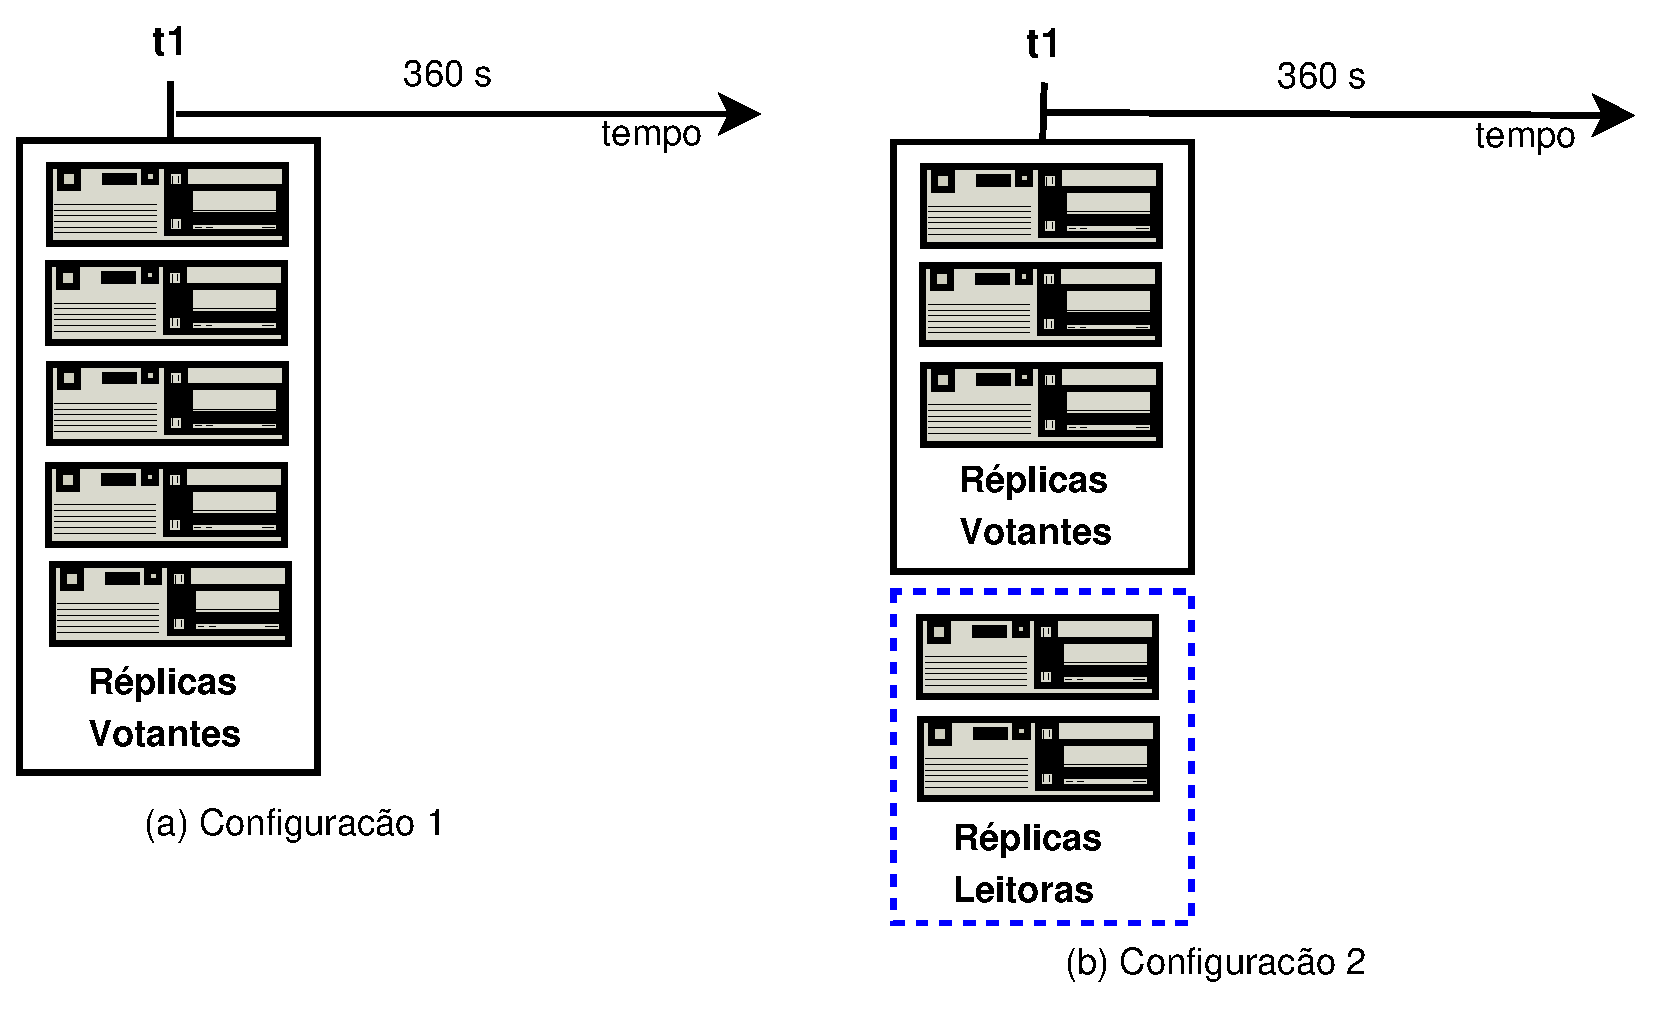
\includegraphics[width=14cm]{conteudo/capitulos/figuras/timeline_exp_leitora.eps}
  \caption{Linha do tempo experimento réplicas leitoras}
  \label{fig:timeline_exp_leitora}
\end{figure}

Nesse cenário a legitimidade na formação de quórum para eleição do consenso durante as
rodadas de Paxos depende da formação utilizada. Na formação 1 não conseguimos consenso
quando três réplicas falham enquanto a formação 2 tolera falha em apenas duas réplicas.
Podemos afirmar então que a tolerância a falhas em Treplica está ligada diretamente como o
número de réplicas votantes existentes na formação do aglomerado, sendo assim, a formação
1 é mais tolerante a falhas.

\subsection{Procedimento de teste}\label{subsec:procedimento_teste_leitora}

Os passos para execução do experimento para medir o desempenho de réplicas leitoras são
listados a seguir:

\begin{enumerate}
  \item Iniciar manualmente o serviço do HAProxy em uma instância dedicada para o serviço
    de \emph{load balancer};
  \item Configurar, através de \emph{script}, as réplicas que atuarão como servidoras,
    respeitando os parâmetros que define se a réplica atuará como votante ou leitora.
    Nesse passo é executado a instalação da JVM e Tomcat (a aplicação de teste foi
    previamente instalada Tomcat);
  \item Configurar, através de \emph{script}, cinco instâncias dedicadas para o serviço de
    cliente. Nesse passo também é instalado a JVM nas instâncias clientes e o programa de
    teste;
  \item Iniciar com \emph{script} o serviço do Tomcat em todas as réplicas servidoras;
  \item Iniciar com \emph{script} o programa de teste nas cinco máquinas dedicadas para
    atuarem como cliente;
  \item Aguardar mais 360 segundos;
  \item Através de \emph{script}, encerrar os processos Javas iniciados (cliente e
    servidor) e recolher os arquivos de \emph{log} dos clientes e servidores.
\end{enumerate}

Aqui, diferentemente do experimento de transferência de estado, iniciamos a aplicação nas
instâncias que atuam como servidoras simultaneamente.

\subsection{Resultados e Análise}

Para análise desse experimento consideraremos as cargas do Experimento 1 e do Experimento
2 que já foram definidas na \autoref{subsec:carga}. Conforme descrito na
\autoref{subsec:procedimento_teste_leitora}, em todas as execuções desse experimento as
réplicas foram iniciadas simultaneamente. Sendo assim, eventuais sobrecargas na
inicialização de réplicas leitoras foram eliminadas pois não existe nenhum estado para ser
transferido. Em outras palavras, no momento que os geradores de carga iniciam todas as
réplicas compartilham do mesmo estado vazio.

Nesse experimento redefinimos o período de análise para 260 segundos de execução. Foram
descartamos os 20 segundos inciais e finais visando eliminar eventuais \emph{outliers}. A
análise de desempenho para esse cenário visa responder uma questão: Qual é o desempenho de
uma réplica leitora?

Para responder essa pergunta, vamos comparar a execução de dois cenários distintos:

\begin{itemize}
  \item Cenário 1: Execução da carga do Experimento 1 (50\% de requisições de leitura)
    em um aglomerado com: (1) 5 réplicas votantes; (2) 3 réplicas votantes e 2 réplicas
    leitoras;
  \item Cenário 2: Execução da carga do Experimento 2 (80\% de requisições de leitura)
    com a mesma formação de aglomerados do Cenário 1;
\end{itemize}

O desempenho do Cenário 1 é ilustrado pela \autoref{fig:replica_leitora_cenario1}.
Analisando os resultados não podemos afirmar qual formação de aglomerado teve o melhor
desempenho. Podemos notar que o desempenho do aglomerado configurado somente com réplicas
votantes (\autoref{fig:replica_leitora_cenario1} (a)) é semelhante ao desempenho do
aglomerado com réplicas leitoras ((\autoref{fig:replica_leitora_cenario1} (b)). O
desempenho das réplicas leitoras nesse cenário é animador, visto que essa é a configuração
experimental que mais exige participação de réplicas votantes.

\begin{figure}[ht]
  \centering
  \includegraphics[width=14cm]{conteudo/capitulos/figuras/final-replica-leitora-pr50.eps}
  \caption{Comparação do desempenho dos aglomerados no Cenário 1}
  \label{fig:replica_leitora_cenario1}
\end{figure}

O mesma análise do Cenário 1 pode ser replicada para o Cenário 2, conforme ilustra a
\autoref{fig:replica_leitora_cenario1}. Novamente nenhuma afirmação pode ser feita sobre
qual é a melhor formação de aglomerado. Esse é mais uma resultado positivo para as réplicas
as leitoras que conseguem se equiparar o desempenho de réplicas votantes e possuem uma
grande vantagem: adição/remoção sem necessidade de reconfiguração total. Essa
flexibilidade no redimensionamento do aglomerado utilizando réplicas leitoras passa a ser
um diferencial a ser explorado em Treplica.

\begin{figure}[ht]
  \centering
  \includegraphics[width=14cm]{conteudo/capitulos/figuras/final-replica-leitora-pr80.eps}
  \caption{Comparação do desempenho dos aglomerados no Cenário 2}
  \label{fig:replica_leitora_cenario2}
\end{figure}

Vamos agora analisar os resultados de uma perspectiva diferente, a
\autoref{fig:analise_final_replica_leitora} ilustra a comparação do número de requisições
suportadas e tempo de respostas nos dois cenários experimentais. Fica evidente a
semelhança no desempenho das duas formações do aglomerado nesses dois critérios.

\begin{figure}[ht]
  \centering
  \includegraphics[width=14cm]{conteudo/capitulos/figuras/final-replica-leitora.eps}
  \caption{Comparação do desempenho de aglomerados com réplicas leitoras}
  \label{fig:analise_final_replica_leitora}
\end{figure}

Para maior clareza de comparação, os resultados ilustrado pela
\autoref{fig:analise_final_replica_leitora} também são exibidos na
\autoref{tab:adicionando_replica_votante} (aglomerado configurado somente réplicas
votantes) e na \autoref{tab:adicionando_replica_leitora} (aglomerado configurado com
réplicas votantes e leitoras).

\begin{table}[htb]
\IBGEtab{
  \caption{Desempenho com réplicas leitoras}
  \label{tab:desempenho_com_replica_leitora}
}{
  \begin{tabular}{ccc}
  \toprule
  Leitura & Operações por Segundo & Tempo de Resposta (ms) \\
  \midrule \midrule
  50\%    & 3118.375              & 251.804                \\
  \midrule
  80\%    & 4314.798              & 176.524                \\
  \bottomrule
\end{tabular}
}{
  \fonte{Produzido pelos autores.}
}
\end{table}

\begin{table}[htb]
\IBGEtab{
  \caption{Desempenho sem réplicas leitoras}
  \label{tab:desempenho_sem_replica_leitora}
}{
  \begin{tabular}{ccc}
  \toprule
  Leitura & Operações por Segundo & Tempo de Resposta (ms) \\
  \midrule \midrule
  50\%    & 3159.908              & 248.718                \\
  \midrule
  80\%    & 4262.307              & 179.123                \\
  \bottomrule
\end{tabular}
}{
  \fonte{Produzido pelos autores.}
}
\end{table}


\section{Conclusão}\label{sec:conclusao}

